
\section{Data Collection and Measurement}
% Discuss the analytical methods used in the study.
% - Refer to relevant data tables.



\subsection{Field Sampling}
Both springs and rain were sampled in the field. Springs were sampled according to locations visited in past expeditions. Rain was collected in a rain gauge along several transects. Both water bodies were measured in the field for temperature, pH and TDS on a Hanna Instruments HI-991300 and and EXTECH DO700. Samples were also titrated using a Hach digital titrator with 0.0625M HCl to calculate the alkalinity of the water following the Gran Method (Gran, 1952). The field measurements were done 24 hours within having been collected.  Six aliquots were collected for each spring for anion, cation, titration, DIC, isotope and archive purposes respectively.  Rain samples had a smaller yield and so only three aliquots were collected, for ion, isotope and archive purposes. Both water body types were filtered through a 0.2$\micro$m PES membrane in a filtration unit prior to bottling. Cation and archive samples were acidified with concentrated HNO$_3$ to give a pH of $\sim$2, keeping the cations in solution. 

%Titration uncertainty!! Use the mean square error of the titration to calculate the uncertainty of the alkalinity.



\subsection{Major and Trace Element Analysis}

Cation concentrations were determined using a Agilent Technologies 5100 Inductively-Coupled Plasma Optical Emission Spectrometer (ICP-OES) using a calibration line made from a Nepalese spring stock solution.
Anion concentrations were determined using a Dionex Ion Chromatography System (ICS) 5000 series against the Battle-02 standard calibration line. Associated uncertainties range between 5-10\% for cations and 10-15\% for anions.

%fact check the anion uncertainty

\subsection{Isotope Analysis}

Samples for radiogenic strontium analysis were dried down to provide at least 10 $\mu$g of Sr. Samples were then dissolved in aqua regia (3:1 HNO$_3$:HCl) to remove any additional organic matter. Once dried down again, they were added to 3 ml teflon columns with Eichrom SrSpec$^{\textcopyright}$ resin pipetted in. Once washed three times with Milli-Q$^{\textregistered}$ water, the column was primed with 3M HNO$_3$. The sample was centrifuged then loaded onto the column avoiding any solids. The column was then washed a total of three times with 3M HNO$_3$ to remove other cations. Lastly, the column was eluted to a beaker with Milli-Q$^{\textregistered}$ water to collect the Sr. Once dried, the samples were dissolved in 3M HNO$_3$, centrifuged and then diluted for analysis on a Thermo Scientific Neptune Plus MC-ICP-MS. Errors on Sr isotope measurement are taken from two standard deviations of the measured values given by the MC-ICP-MS.

\bsk

Samples were also analysed for stable oxygen and deuterium isotopes on a Picarro L2140-i portable analyser, using cavity ring-down spectroscopy, with an average precision of 0.05, 0.09 and 0.57 \textperthousand\ for $\delta^{17}O$, $\delta^{18}O$ and $\delta D$ respectively. 


\section{Methods and Models for Analysis}


\subsection{Cyclic and Hydrothermal Correction}

Rain input is a significant factor in the chemical composition of groundwater and rivers. Most chloride found in these water bodies is thought to be due to rainwater input (Drever, 1997). It is standard practice to correct for this cyclic input. Spring water is corrected for rain input according to the average concentration for the closest rain sample collected in this field season. To remove the contribution of the rain the following formula is used for any element X:

%Whilst it would be best to perform a temporal correction, a spatial correction where the rain is collected from the same catchment as the analysed spring samples is already a significant improvement over the current literature (Bickle, 2015 AJS).


\begin{equation}
    [X]_{rain-corrected}  = [X]_{river} - (Cl_{river} - Cl^*_{river})\frac{[X]_{rain}}{[Cl]_{rain}}
\end{equation}
\begin{equation}
    Cl^*_{river} = Cl_{river} - Cl_{rain}; \quad \text{if} \quad Cl_{river} > Cl_{rain}
\end{equation}\\
    

Where $[Cl]^*_{river}$ is is calculated by subtracting the concentration of chloride in the rain from that in the river (Tipper et al, 2006). $Cl^{*}$ is taken to be zero if the concentration of chloride in the rain is greater than concentration of river. Evapotranspiration is not considered by this model, and studies which show that it plays a minor role, accounting for less than 10\% of the hydrological budget in the Himalayas (Andermann et al (2012); Bookhagen and Burbank, 2010). In those cases where $Cl^*$ is not zero then, a primary rain correction is simply:

\begin{equation}
[X]_{rain-corrected}  = [X]_{river} - [X]_{rain}
\end{equation}\\

Once the samples have been corrected for rain input, the remaining $[Cl]^{-}$ is assumed to be derived from hydrothermal springs encountered in the flow path. This is likely to be the case in one of the southern traverses (Traverse 2) in Melamchi which display high chloride concentrations even after the cyclic correction. Hence, the sample with the highest $[Cl]^{-}$ is used to correct:

\begin{equation}
[X]_{hydrothermal-corrected}  = [X]_{rain-corrected} - \frac{[X]}{[Cl]}_{highest-Cl} * [Cl]_{rain-corrected}
\end{equation}\\

This ensures that all chloride in the corrected sample is removed. The correction uses ionic ratios from the most concentrated water source, which acts as a proxy for the sediment imparting its signature.  In this way, the correction does not affect samples which do not have high Cl (and hence do not have a large hydrothermal contribution), but does decrease the concentration of ions for those that do. In the following sections, samples are plotted with the evaporite correction applied where possible. Only in those cases where no chloride was measured is the evaporite correction not applied.

\newpage

\subsection{Modal Decomposition Identifies Weathering Reaction}

The first step towards quantifying the extent to which chemical weathing reactions have gone to completion is to discern what reaction is taking place. In principle this is as simple as knowing what minerals are dissolving and which are precipitating. Modal decomposition methods consider several minerals that could be dissolving and/or precipitating, and their stoichiometry (Garrels and Mackenzie, 1967; Drever, 1997). Note that this calculation can only be done if the number of components is the same as or greater than the number of minerals.


\begin{center}
\[
  \begin{bordermatrix}
{ & Biot & Plag & Calc & Smec & Kaol & KSpar \cr
Si  & a_{11}  & a_{12}  & a_{13}  & a_{14}  & a_{15}  & a_{16}  \cr
Al  & a_{21}  & a_{22}  & a_{23}  & a_{24}  & a_{25}  & a_{26}  \cr
Mg  & a_{31}  & a_{32}  & a_{33}  & a_{34}  & a_{35}  & a_{36}  \cr
Ca  & a_{41}  & a_{42}  & a_{43}  & a_{44}  & a_{45}  & a_{46}  \cr
Na  & a_{51}  & a_{52}  & a_{53}  & a_{54}  & a_{55}  & a_{56}  \cr
K   & a_{61}  & a_{62}  & a_{63}  & a_{64}  & a_{65}  & a_{66}  \cr}
  \end{bordermatrix}
  \cdot
  \begin{bordermatrix}
{ &  \cr
  & x_{Biot} \cr
  & x_{Plag} \cr
  & x_{Calc} \cr
  & x_{Smec} \cr
  & x_{Kaol} \cr
  & x_{KSpar} \cr}
  \end{bordermatrix}
  =
  \begin{bordermatrix}
{ & Spring (\mu mol/l) \cr
  & b_1 \cr
  & b_2 \cr
  & b_3 \cr
  & b_4 \cr
  & b_5 \cr
  & b_6 \cr}
  \end{bordermatrix}
\]
\end{center}
\bsk

Matrix algebra facilitates the calculations of the mineral proportions in the water. Given known matrices \( A \) and \( B \), where A represents the stoichiometric quantities of elements in a mineral, and B the concentrations of elements in the water:

\begin{equation}
AX = B
\end{equation}
\begin{equation}
X = A^{-1}B
\end{equation}\\

The matrix X, corresponding to volumetric proportions of the minerals in the water, can then be calculated, under the assumptions that all minerals dissolve in a congruent fashion. Modal decompostion for spring waters was performed according to stoichiometric proportions from Bickle et al. (2015). For ease of visualisation, Figure \ref{fig:discussion6} shows the positive, dissolved minerals on the LHS, and the negative, precipitated minerals on the RHS.\\

\begin{figure}[h]
    \centering
    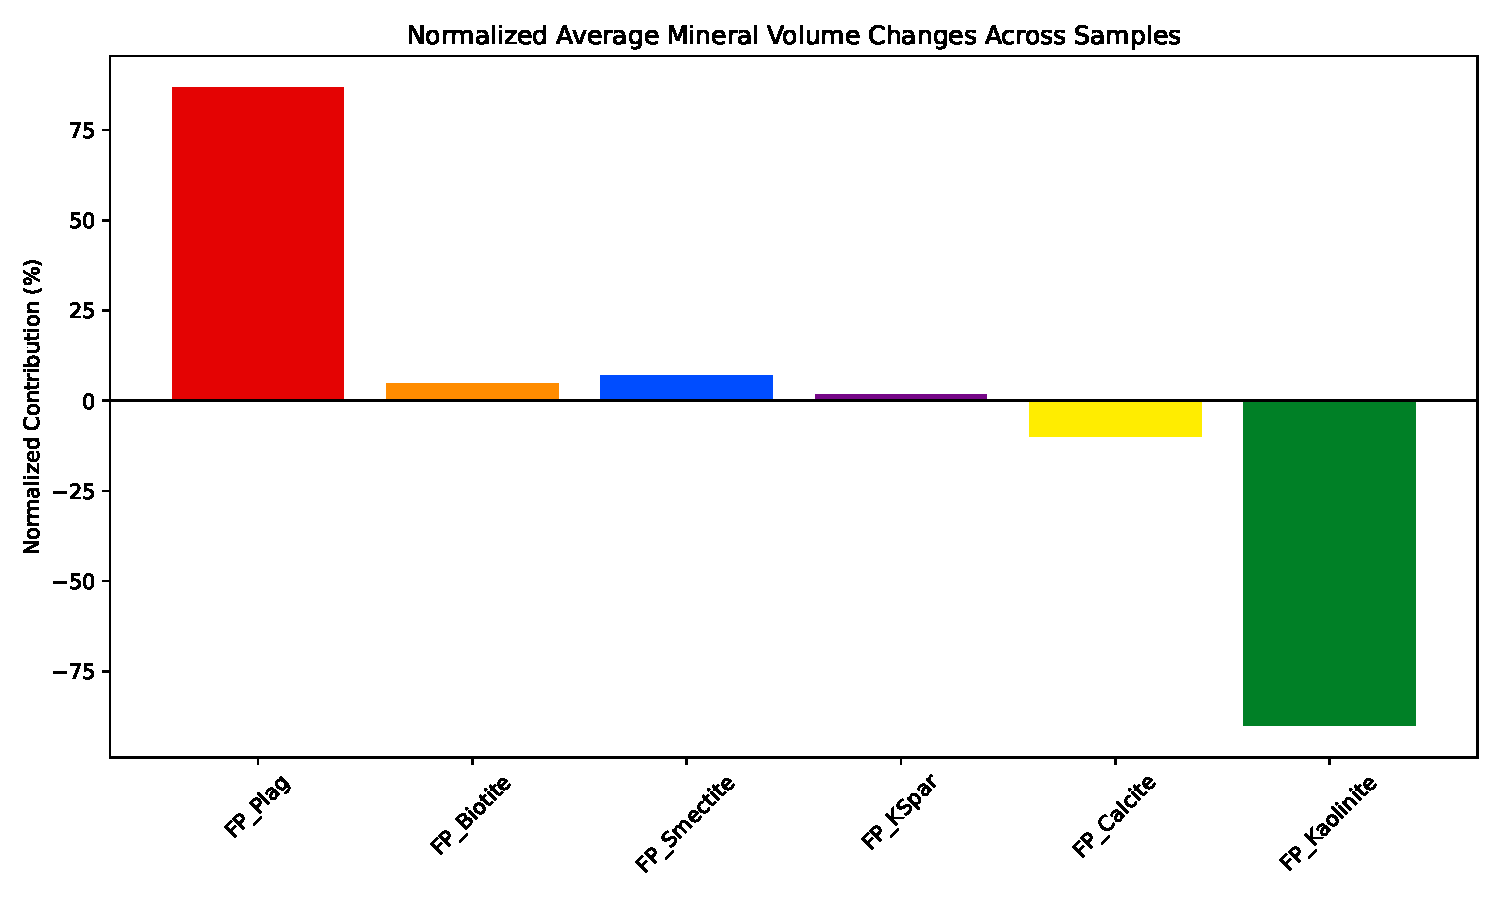
\includegraphics[width=\textwidth]{Stoich.pdf}
    \caption{Average of the modal decomposition for the springs in Traverse 3.}
    \label{fig:discussion6}
\end{figure}

\FloatBarrier

Figure \ref{fig:discussion6} is representative of most springs in Traverse 3. Hence, the major phase being dissolved is plagioclase feldspar and the major phase being precipitated is kaolinite. The primary composition of plagioclase in the area corresponds to $\approx$ An-20 (Bickle et al., 2015; Knight et al., 2024).  The plagioclase to kaolinite reaction is given by the following equation (written so that aluminium is conserved):

\begin{equation}
    \begin{matrix}
Ca_{0.20}Na_{0.80}Al_{1.20}Si_{2.80}O_{8} + 1.2H^{+} + 0.6 H_{2}O \\ \rightarrow\\ 0.6 Al_{2}Si_{2}O_{5}(OH)_{4} + 0.8 Na^{+} + 0.2 Ca^{2+} + 1.6 SiO_{2}(aq)
    \end{matrix}
\end{equation}
\quad Or
\begin{equation}
    \begin{matrix}
An_{20} + 1.2 H^{+} + 0.6 H_{2}O\\ \rightarrow\\ 0.6 Kaolinite + 0.8 Na^{+} + 0.2 Ca^{2+} + 1.6 SiO_{2}(aq)
\end{matrix}
\label{eq:10}
\end{equation}\\


\subsection{One-Dimensional Reactive Transport Models}

Reactive transport models are widely used in applied fluid dynamics and various fields within Earth Sciences. These models aim to track chemical reactions occurring at each spatial point, accounting for the movement of reactants to and reaction products away from those points (Bethke, 2011). The basic form of a reactive transport model is a partial differential equation that describes the transport of solutes and the reactions that occur between them. For reacting solutes, concentration changes over time are governed by transport rates — derived from the divergence principle — and the relative rates of dissolution and precipitation (Bethke, 2011). The proposed equations can be complex, but in simple cases a species of concentration $C_i$ can be modelled to follow a first-order rate law, generally represented by:

\begin{equation}
    \frac{\partial C_i}{\partial t} = \mathcal{O}_{T}(C_i) + \mathcal{O}_{R}(C_i)
    \label{eq:1}
\end{equation}\\


Where \(\mathcal{O}_{T}\) and \(\mathcal{O}_{R}\) are the transport and reaction operators, respectively (Bethke, 2011). Depending on the hypothesis supported, equation \ref{eq:1} can be modified accordingly. The following sections will discuss two models with their own versions of equation \ref{eq:1}.



%Also need to make a mini 1D graphic explaining what the 1D model actually means in practice


\subsubsection{Model Motivation}

As discussed in the Introduction (ref), there are different hypotheses regarding the major controls on chemical weathering. This section will contrast one model following the null hypothesis that weathering is largely sensitive to climate and temperature (Fontorbe et al., 2013), and another model that suggests weathering is more sensitive to fluid flux (Maher, 2011; Maher and Chamberlain, 2013). Given the emphasis on deriving fluid residence times from solute concentrations, the benchmark for a model's effectiveness will be how well it can predict these times compared to previous studies on gas tracers and simple box models. Assumptions and constraints will be compared and contrasted, and their results used to inform the calculation of rates of reaction and approach to equilibrium in Melamchi. For both models, the element used to benchmark is dissolved silicon. This is because silicon is present in both dissolution and precipitation reactions, so it is applicable to the Maher model which considers both reactions. Furthermore, silicon is what both models were used for in their respective original studies.

\newpage

\subsubsection{Fontorbe et al. (2013) - Model}

This model investigates silicon isotopic composition in the Ganges River, assuming constant reaction rates along flow paths (see Appendix for a full derivation, and Table ref for a list of parameters used). The first-order differential equation governing transport and reaction is given as:\\

    \begin{equation}
    \phi \frac{\partial C}{\partial t} = -\omega \phi \frac{\partial C}{\partial z} + R_n(1-f)
    \end{equation}\\

Where C is the elemental concentration, $\omega$ is the fluid velocity, $\phi$ is the rock porosity, z is a position along the flow path, R$_\text{n}$ is the rate of reaction, and f is the fraction of Si present in the dissolved load that is reprecipitated in the back reaction. The equation can be nondimensionalised using the Damköhler number (\(N_D\)), which describes the relative importance of kinetic vs transport-controlled settings (Bethke, 2008):\\

\begin{equation}
    N_D = \frac{R_n h}{\phi C_0 \omega}
\end{equation}\\

Assuming steady-state (\(\partial C/\partial t = 0\)), the concentration at the end of the flow path can be rearranged to give the residence time \(T_f\):\\

\begin{equation}
    T_f = \frac{(C - C_0)\phi}{(1-f)R_n}
\end{equation}



\newpage

\begin{table}[H]
    \centering
    \renewcommand{\arraystretch}{1.3} % Adjust row height
    \begin{tabular}{|c|c|c|c|}
        \hline
        \multicolumn{4}{|c|}{\textbf{Fontorbe}} \\  
        \hline
        \textbf{Parameter} & \textbf{Definition} & \textbf{Units} & \textbf{Formula (Value)} \\  
        \hline
        $\phi$ & Porosity & - & 0.1 $^*$\\
        $\omega$ & Fluid velocity & m/s & Variable \\
        $h$ & Length of flow path & m & Variable \\
        $C$ & Concentration \@ end of flow path & $\mu$mol/L & Variable \\
        $C_0$ & Initial concentration & $\mu$mol/L & Rain Input \\
        $f$ & Fraction reprecipitated & - & 0.5$^*$ \\
        $N_D$ & Damkohler Number & - & $N_D = \frac{R_n h}{\phi C_0 \omega}$ \\
        $T_f$ & Residence time & s & $T_f = \frac{h}{\omega\phi}$ \\
        $R_n$ & Reaction rate & mol/m$^3$/s & $\rho \cdot 10^6 \cdot k \cdot S \cdot X $ \\
        $k$ & Reaction rate constant & mol/m$^2$/s & 10$^{-15*}$ \\
        $S$ & Specific surface area & m$^2$/g & 0.1$^*$ \\
        $\rho$ & Plagioclase density & g/cm$^3$ & 2.7$^*$ \\
        $X$ & Volume fraction of mineral in rock & $g_{min}/g_{rock}$ & 0.2$^*$ \\
        \hline
    \end{tabular}
    \caption{Key parameters and definitions for the Fontorbe model. Starred terms are values used for calculation.}
    \label{tab:parameters1}
\end{table}


\FloatBarrier









\newpage




\subsubsection{Maher and Chamberlain (2014) Model}


This model is built in accordance with the principle that the main control on silicate weathering is the residence time of the water. The model is based on the assumption that the reaction rate decreases linearly with approach to equilibrium, and that all weathering paths approach equilibrium. The motivation behind the hydrological control is based on sensitivity analyses of real catchment data on one-dimensional reactive transport models which suggest that porosity, mineral surface area, and temperature have no consistent correlation with water composition (Maher, 2011). See Appendix and Table ref for a full derivation and the model parameters respectively. The model begins with the following representation of the concentration of a solute in a fluid flow path:\\ 

\begin{equation}
    \frac{dC}{dt} = -\frac{q}{\theta} \frac{dC}{dz} + \sum_i \mu_i R_{d,i} \left( 1 - \left( \frac{C}{C_{eq}} \right)^{n_i} \right)^{m_i} - \sum_i \mu_i R_{p,i} \left( 1 - \left( \frac{C}{C_{eq}} \right)^{n_i} \right)^{m_i}
\end{equation}

Where \( C \) is the concentration, \( q \) is the fluid flux, \( \theta \) is the volumetric water content, \( z \) is the position along the flow path, \( \mu \) is the stoichiometric coefficient, \( R \) is the rate of reaction for dissolution and precipitation respectively, \( C_{eq} \) is the equilibrium concentration, and \( n \) and \( m \) are non-linear parameters (Maher and Chamberlain, 2013). For a given packet of water, R$_{\text{n}}$ is defined as: \\

\begin{equation}
R_n = R_{d} - R_{p}
\end{equation} 
\begin{equation}
\frac{dc}{dt} = R_n \left( 1 - \frac{C}{C_{\text{eq}}} \right)
\end{equation} \\

Where R$_d$ and R$_p$ are the rates of dissolution and precipitation respectively. This can be solved for concentration, and rearranged for residence time to obtain:\\

\begin{equation}
    T_f = \frac{C_{eq} \cdot \left(C - C_0\right)}{e^2 R_n \left( C_{\text{eq}} - C \right)}
\end{equation}\\

Note the $e^2$ term is used because the Maher model considers all paths as if they approach equilibrium.

\begin{table}[H]
    \centering
    \renewcommand{\arraystretch}{1.3} % Adjust row height
    \begin{tabular}{|c|c|c|c|}
        \hline  % DOUBLE BOLD LINE
        \multicolumn{4}{|c|}{\textbf{Maher}} \\  
        \hline
        \textbf{Parameter} & \textbf{Definition} & \textbf{Units} & \textbf{Formula (Value)} \\  
        $\phi$ & Porosity & - & 0.1$^*$ \\
        $h$ & Length of flow path & m & Variable \\
        $q$ & Flow rate & m/s & Variable \\
        $C_{eq}$ & Equilibrium concentration & $\mu$mol/L & Max Catchment \\
        $C_0$ & Initial concentration & $\mu$mol/L & Rain Input \\
        $R_n$ & Net reaction rate & mol/L/s & $\rho \cdot 10^6 \cdot k \cdot S \cdot X $ \\
        $\rho$ & Plagioclase density & g/cm$^3$ & 2.7$^*$ \\
        $k$ & Reaction rate constant & mol/m$^2$/s & 10$^{-15*}$ \\
        $S$ & Specific surface area & m$^2$/g & 0.1$^*$ \\
        $X$ & Volume fraction of mineral in rock & $g_{min}/g_{rock}$& 0.2$^*$ \\
        $\tau$ & Scaling factor & - & $\tau = e^2$ \\
        $D_w$ & Damkohler Coefficient & m$^2$/s & $D_w = \frac{L \phi R_n}{C_{\text{eq}}}$ \\
        $T_f$ & Residence time & s & $T_f = \frac{h \phi}{q}$ \\
        \hline
    \end{tabular}
    \caption{Key parameters and definitions for the Maher model. Starred terms are values used for calculation.}
    \label{tab:parameters2}
\end{table}

\FloatBarrier


\subsection{Estimates of Uncertainty}

Uncertainties were propagated using a Monte Carlo method. This leverages randomness to calculate uncertainties. Both observed and estimated parameters have uncertainties associated with them. Each Monte Carlo simulation randomly varies the input parameters within their estimated uncertainty ranges. Once many simulations have been run, the distribution of results reflects the possible range of values obtained for a given relationship. The uncertainty is then calculated as two standard deviations of the mean of the distribution.
